\documentclass{egee-hacked}
\usepackage{comment}
\usepackage{longtable}
\usepackage{makeidx}

\newenvironment{method}[2][]{{\vspace{4mm}\sf #2}\index{operation!
#2}\label{op:#1#2}
\par\nopagebreak\begin{tabular}{p{5mm}p{3mm}p{70mm}p{75mm}}}{\end{tabular}\\[2mm]}
\newcommand{\inpar}[2]{&$\Rightarrow$&\sf #1&#2\\}
\newcommand{\outhead}[2]{&$\Leftarrow$&\sf #1&#2\\}
\newcommand{\outpar}[2]{&&\sf #1&#2\\}
\newcommand{\faults}{}
\newcommand{\desc}{\end{tabular}\par\begin{tabular}{p{5mm}p{150mm}}
\\[-3mm] &} 
\newcommand{\OK}{
	\outhead{Tuple(1..1)}{}
	\outpar{xsd:string status}{OK}
}

\makeindex

\title{R-GMA System Specification Version}
\Version{6.2.0}
\Date{\today}
\Dissemination{PUBLIC}
% \DocumentLink{http://edms.cern.ch/document/490223/}

\Abstract{
This document presents the System Specification for the Information and 
Monitoring Services middleware component (R-GMA) in sufficient detail to 
support design verification, detailed design and test specification. It 
specifies precisely the interfaces and externally visible behaviour of all the 
R-GMA services.

The document is structured with a single chapter containing a technical
overview of the system, followed by a separate chapter for each of
the R-GMA services, with a standard set of headings in each of these chapters.
Chapters on security, SQL language support, service data types and
service parameters complete the document.}

\begin{document}

%
% Official text received on October 6, 2004
%
\vspace*{\fill}{\bf Copyright }\copyright{\bf Members of the EGEE Collaboration.
2004. See http://eu-egee.org/partners for details on the copyright holders. 

EGEE (``Enabling Grids for E-science in Europe'') is a project funded by
the European Union.  For more information on the project, its partners
and contributors please see http://www.eu-egee.org.

You are permitted to copy and distribute verbatim copies of this
document containing this copyright notice, but modifying this document
is not allowed. You are permitted to copy this document in whole or in
part into other documents if you attach the following reference to the
copied elements: ``Copyright }\copyright{\bf 2004. Members of the EGEE
Collaboration. http://www.eu-egee.org''

The information contained in this document represents the views of
EGEE as of the date they are published. EGEE does not guarantee that
any information contained herein is error-free, or up to date.

EGEE MAKES NO WARRANTIES, EXPRESS, IMPLIED, OR STATUTORY, BY
PUBLISHING THIS DOCUMENT.}




\newpage
\tableofcontents

\newpage
\section{Introduction}
\label{sec:Introduction}

\subsection{Purpose and Structure of this Document}

This document presents the more important aspects of the design for the Information
and Monitoring Services middleware component (R-GMA) where it is not convenient
to use comments in the code. 

The various sections describe different parts of the system.

It is suggested that you read first about the Primary Producer Service
in Section \ref{sec:primaryProducerService} and then from the Request
Management Subsystem in Section \ref{sec:requestManagementSubsystem}
down to and including the Remote Call Subsystem in Section
\ref{sec:remoteCallSubsystem}.

\newpage
\section{Message Formats}\label{sec:MessageFormat}

\subsection{Data types}

An important part of these chapters is the list of operations and their input 
and output parameters. Input parameters are prefixed by $\Rightarrow$ and 
output parameters by $\Leftarrow$. Parameters may be omitted or repeated as
indicated by the notation:

\begin{description}
\item[(1..1)] Exactly once - the default
\item[(0..1)] May be omitted
\item[(1..*)] At least one
\item[(0..*)] Any number
\end{description}

after the basic type name. Types take the following values:

\begin{description}
\item[xsd:string] a sequence of Unicode characters
\item[xsd:boolean] the literals \textit{true} or \textit{false} encoded as strings
\item[xsd:int] an integer in the range $[-2^{31},2^{31} -1]$
\item[xsd:long] an integer in the range $[-2^{63},2^{63} -1]$
\item[Tuple] a tuple. This is followed by a list of the fields within the tuple.
These can be of any of the types mentioned - except for another tuple.
\end{description}

\subsection{Request}

Simple requests (such as xsd:string) values are sent as http request parameters 
(either POST or GET) and Tuples are encoded as one or more result sets within 
an XML string sent as a single http parameter. 

\subsection{Response}

The output is sent as an XML encoding of one or more R-GMA tuple sets. 

Errors are also encoded as XML.

\subsection{XML formats}

\subsubsection{Tuple set}\label{sec:TupleXML}

A single result set looks like:

\begin{verbatim}
<r m="Be warned" r="2" c="2">
  <v>Row 1 Col 1</v>
  <v>Row 1 Col 2</v>
  <n/>
  <v></v>
  <e/>
</r>
\end{verbatim}

The result set has an (optional) and has 2 rows and 2 columns as indicate by the
r and c attributes which default to 1. The data values then follow inside
\verb!<v></v>! or \verb!<n/>! to indicate the null value. The \verb!<e/>!
indicates that there is no more data.

With these rules a simple ``OK'' message is just

\begin{verbatim}
<r><v>OK</v><e/></r> 
\end{verbatim}

Multiple tuple sets must be wrapped in \verb!<s></s>! as shown below:

\begin{verbatim}
<s>
  <r><v>OK</v><e/></r> 
  <r><v>OK</v><e/></r>
</s> 
\end{verbatim}

\subsubsection{Errors}

A temporary exception is represented as:

\begin{verbatim}
<t m="This may recover" o="1"/>
\end{verbatim}

where the o attribute shows the number of succesfgul operations and defaults to
0.

A permanent exception uses p instead of t. For example:

\begin{verbatim}
<p m="This will not recover"/>
\end{verbatim}

The unknown resource message is very simple - it is just:

\begin{verbatim}
<u/>
\end{verbatim}




\newpage
\section{Primary Producer Service}\label{sec:PrimaryProducer}\index{primary producer}

\subsection{Description}

Primary Producer resources are created by the Primary Producer Service
at the request of a user who wishes to publish tuples into to one or
more tables in a virtual database\index{virtual database}.
The principal components of a
Primary Producer resource are shown in the picture below. They contain
tuple stores\index{tuple store} to hold tuples inserted by the user,
and they have an SQL query processor to run consumer queries against
their tuple stores. They are the primary source of data in a virtual
database. They all support continuous queries, and can be configured
to support any combination of latest and history queries as well.

\begin{center}
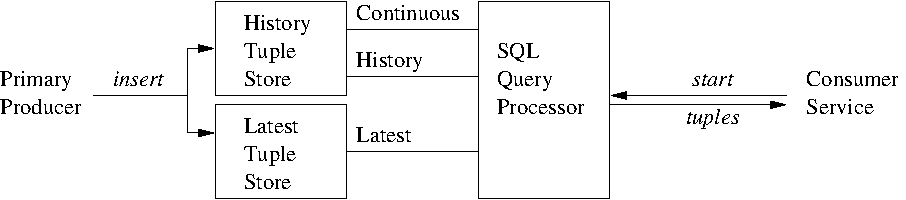
\includegraphics[width=145mm]{pp_detail}
\end{center}

The Primary Producer Service is responsible for authenticating all users and
services that connect to it, and for authorizing all operations and all requests
to access its tuple stores, as specified in chapter~\ref{sec:Security}.

\subsection{Interface}

\subsubsection{User Interface}

\begin{method}{createPrimaryProducer}
\inpar{xsd:boolean isHistory}{If history queries are supported}
\inpar{xsd:boolean isLatest}{If latest queries are supported}
\inpar{xsd:string type} {DATABASE or MEMORY}
\inpar{xsd:string logicalName}{The logical name should not be
be specified for type MEMORY. For type DATABASE it is optional.} 
\outhead{Tuple(1..1)}{}
\outpar{xsd:int connectionId}{connectionId of new Primary Producer resource.} 
\desc
Creates a new Primary Producer resource and returns its endpoint. The
Primary Producer is not added to a Registry until
\textit{declareTable} is called. The user cannot prevent Primary
Producers from supporting continuous queries, but support for latest
and/or history queries is optional. Primary Producers can use any type
of storage, regardless of the query types they support. Tuple stores can be
made permanent by providing a \textit{logical name} for the tuple store as
described in \ref{sec:PrimaryProducerTupleStores}. The termination interval is
described in \ref{sec:PrimaryProducerCreating}.
\end{method}

\begin{method}{declareTable}
\inpar{xsd:int connectionId}{Primary Producer resource identifier.}
\inpar{xsd:string tableName}{VDBTable to register.}
\inpar{xsd:string predicate}{Producer's predicate.}
\inpar{xsd:int hrpSec}{History Retention Period in seconds.}
\inpar{xsd:int lrpSec}{Latest Retention Period in seconds.}
\OK
\desc
Adds a table to the list of tables to which this producer may publish tuples,
as described in \ref{sec:PrimaryProducerDeclaring} below. The table name must
have an explicit virtual database name prefix (separated from it by a dot).
The format of the predicate is specified in \ref{sec:SQLPredicates}, and
the retention periods are described in \ref{sec:PrimaryProducerRemoving} (the 
latest retention period can be overridden in \textit{insert}). 
\end{method}

\begin{method}{insert}
\inpar{xsd:int connectionId}{Primary Producer resource identifier.}
\inpar{xsd:string insert}{SQL INSERT statement.}
\inpar{xsd:int(0..1) lrpSec}{Latest Retention Period in seconds.}
\OK
\desc
Inserts one or more tuples into a primary producer resource's tuple stores, as
described in \ref{sec:PrimaryProducerInserting}. The format of the insert
statement is specified in \ref{sec:SQLInsert}; as with \textit{declareTable},
the table name must have an explicit virtual database name prefix. Inserted
tuples must match the producer's predicate and the table schema or they will be
rejected. If the latest retention period is omitted, the default specified in
the call to \textit{declareTable} will be used. If a tuple is found to be invalid or cannot
be inserted for any reason, the operation will stop and throw an
RGMAException indicating the number of tuples successfully inserted in
its \textit{numSuccessfulOps} field (those tuples will remain in the tuple
stores).
\end{method}

\begin{method}{getLatestRetentionPeriod}
\inpar{xsd:int connectionId}{Primary Producer resource identifier.}
\inpar{xsd:string tableName}{VDBTable name.}
\outhead{Tuple(1..1)}{}
\outpar{xsd:int hrpSec}{Latest Retention Period in seconds.}
\desc Returns a Primary Producer resource's declared Latest Retention Period for
a given table.
\end{method}

See also the common producer service operations:
getHistoryRetentionperiod~\ref{op:getHistoryRetentionPeriod}.

See also the common resource management service operations:
close~\ref{op:close} and
destroy~\ref{op:destroy}.

See also the operation common to all services:
getProperty~\ref{op:getProperty}.

\subsubsection{System Interface}

See  the common producer service operations:
start~\ref{op:start} and abort~\ref{op:producerabort}.

See the common resource management service operation:
ping~\ref{op:resourceping}.

\subsection{Details}
\subsubsection{Creating and destroying Primary Producers}\label{sec:PrimaryProducerCreating}

A new Primary Producer Resource is created when a user calls the
\textit{createPrimaryProducer} operation and is destroyed when the
user calls the \textit{close} or \textit{destroy} operations. The
special processing for \textit{close} is desribed below. In addition,
if the service does not hear from the user for a period exceeding the
\textit{termination interval}\index{termination interval}, the service
will initiate a \textit{close} operation on the resource. A call to
any user operation on the resource is sufficient to keep it alive.

\subsubsection{Tuple stores}\label{sec:PrimaryProducerTupleStores}\index{tuple store}

The Primary Producer's history and latest tuple stores were described in 
\ref{sec:BackgroundTupleManagement}. They may be physically in memory or 
database storage. The memory storage may also make use of an RDBMS (typically 
memory resident) but is transient. A single producer uses 
only one type of storage for all types of queries that it supports.

The Primary and Secondary Producer services only uses stores created and 
managed by themselves. Tuple stores are normally temporary and are destroyed 
along with the producer resource, but users can make atuple store with database 
storage permanent by specifying a \textit{logical name} for the tuple store 
when they create a new Primary (or Secondary) producer. If the service is 
running in secure mode, the user's Distinguished Name (DN) is prefixed to the 
logical name. In insecure mode, the user must make the name unique within the 
service by some other means. Permanent tuple stores are not destroyed when a 
producer resource is destroyed, so they can be re-used by creating a new 
producer and naming the same store, provided there are no other producers using 
it already. The user can then re-declare any table that is already in the store 
(with a compatible predicate - see \ref{sec:SQLPredicates}) and any existing 
tuples will be automatically recovered. The names and some information about 
tuple stores can be obtained by calling \textit{listTupleStores}. Permanent tuple 
stores are deleted by calling \textit{dropTupleStore}. R-GMA only allows the 
the \textit{owners} of existing tuple stores to re-use or list them.

\subsubsection{Declaring tables}\label{sec:PrimaryProducerDeclaring}\index{declare table}

Producers must declare their intention to publish to a table by calling
\textit{declareTable} before they can insert tuples. The table definition must
already exist in the schema (see \ref{sec:SQLCreateTable}). The Primary
Producer Service obtains the table
definition from the schema by calling \textit{getFullTableDetails} and creates
the corresponding table in the resource's tuple stores (or if it already exists
in a named tuple store, checks its structure). If the
schema specifies that the table should be indexed, the producer creates the
indexes if possible, and also indexes the \textit{RgmaTimestamp} column (see
below).  It then registers the producer as a publisher for
that table, by calling the registry's \textit{registerProducerTable} operation.
The service must be ready to service consumer queries against the resource's
tuple stores as soon as this notification is sent.
This registry operation returns a list of any relevant continuous consumers
and the producer service must send an \textit{addProducer} message to each of
them to notify them about the new producer.
The producer service will also periodically re-send the
\textit{registerProducerTable} to the registry on the user's behalf, to
maintain the producer's entries in the registry throughout its lifetime. The
list of consumers returned is used to help check that consumers are still alive
(see \ref{sec:PrimaryProducerStoppingQueries}).
The user can declare more than one table in a single producer, and these can
even be in different virtual databases. All the tables are treated
independently by the producer service, except for processing ``join'' queries.

\subsubsection{Inserting tuples}\label{sec:PrimaryProducerInserting}\index{insert}

Tuples are inserted into the producer service's tuple storage by calling the
\textit{insert} or \textit{insertList} operations. They are checked for type
against the schema, and for content against the producer's declared predicate.
The following metadata is added to each tuple by the service:

\bigskip\begin{tabular}{llp{95mm}}
MeasurementDate&DATE&This and the next column will be supported for a while for
backward compatibility. At some stage they will be turned into user columns so
that they can be eliminated.\\
MeasurementTime&TIME&See above\\
RgmaTimestamp&TIMESTAMP(9)&
UTC tuple time-stamp: only added by R-GMA if not already filled in by the user;
those added by R-GMA will only have a resolution of 1ms
(see \ref{sec:SQLDataTypes} for the format of a TIMESTAMP)\\
RgmaLRT&TIMESTAMP(6)&
UTC Latest Retention Time (see below)\\
RgmaOriginalServer&VARCHAR(255)&
Hostname (including domain name) of server publishing the information.\\
RgmaOriginalClient&VARCHAR(255)&
Hostname (including domain name) of client publishing the information.\\
\end{tabular}\par\bigskip

Tuples are inserted to the tuple stores and streamed to subscribed consumers
as described in \ref{sec:BackgroundTupleManagement}. If one of the producer's
tuple stores fills up, the service temporarily blocks inserts by returning
an RGMABufferFullException until tuples expire and can be removed, as
described below.

A Producer making use of a named tuple store should avoid sending tuples that
have already been sent by another producer that used the store previously.

\subsubsection{Removing tuples}\label{sec:PrimaryProducerRemoving}\index{History Retention Period}

The user must set a \textit{History Retention Period (HRP)} and a 
\textit{Latest Retention Period (LRP)} for each declared table. The HRP is 
recorded in the registry indicating to the mediator the maximum age of tuples 
it guarantees to maintain in its history tuple store. The Primary Producer 
Service adjusts the HRP it sends to the registry to take account of the actual 
age of its history tuple store (which will be very short for a new producer), 
and updates it in the periodic calls to \textit{registerProducerTable} up to 
the value set by the user as time progresses. The LRP\index{Latest Retention 
Period} is used to calculate a \textit{Latest Retention Time 
(LRT)}\index{Latest Retention Time}\index{LRT|see{Latest Retention Time}} for 
each tuple by adding it to the tuple's RgmaTimestamp (the table-default LRP may be 
overridden in each call to \textit{insert}). The LRT is written into the 
tuple's metadata because Secondary Producers must also respect it. The two 
retention periods are independent. A history tuple store records the time of
insertion of each tuple into the tuple store and uses this to work out when the
tuples should be expired. The same rule applies to a tuple arriving in a tuple
store managed by a secondary producer.

Tuples that have expired in either tuple store can be removed by the service,
and the service is obliged to periodically clean up: it is not allowed to run
out of storage and block inserts if it could free up storage by deleting
expired tuples. In addition, tuples in the latest tuple store that have
exceeded their LRT must \textit{never} take part in latest queries.

The distinction between \textit{close}\index{close} and
\textit{destroy}\index{destroy} on a Primary Producer is that a \textit{close} 
will wait for tuples to be streamed to any continuous consumers that have not 
yet received them, and will also wait for any tuples in a memory based history 
tuple store to expire before the producer is destroyed. Note that the wait for 
tuples to expire does not apply to the latest tuple store nor to tuple stores 
using database storage. During this time, the producer will remain registered 
and still accept new history queries and latest (but not new continuous 
queries) for each declared table until all tuples for the table have expired 
from the history tuple store, at which point the corresponding table is 
unregistered, by calling \textit{unregisterProducerTable}. When all tables have 
been unregistered and all tuples have been streamed, the producer resource is 
destroyed.

\subsubsection{Processing queries}\label{sec:PrimaryProducerQueryProcessing}

Consumer services send a \textit{start} message to a Primary Producer
to request it to execute a query and start streaming the resulting
tuples back to the consumer service. Continuous queries receive all old tuples
available in the producer's history store since the start time specified in the
\textit{start} call, followed by all new tuples as they are inserted to the
producer. One-time queries execute on the current
contents of the history and latest tuple stores only and terminate when they've
returned all of the results to the consumer service.

The streaming protocol and the streaming server in the consumer service are
described in section \ref{sec:ConsumerStreaming}. As described there, tuples
are streamed in \textit{chunks}, with the last chunk for a one-time query
distinguished by an \textit{end-of-results} flag.
The connection details of the streaming server, and the maximum
number of tuples it will accept in a single chunk, are passed in the
\textit{start} call. It is the responsibility of the implementation to ensure
that the results of a one-time query are evaluated just once and are immune to
changes to the tuple stores while the results are being streamed.

\subsubsection{Stopping queries}\label{sec:PrimaryProducerStoppingQueries}

One-time queries automatically terminate when the last tuple has been
streamed to the consumer. All queries may be terminated by running
for longer than the query \textit{timeout} specified in the call to
\textit{start}.

\newpage
\section{Secondary Producer Service}\label{sec:SecondaryProducer}\index{secondary producer}

\subsection{Description}

Secondary Producer resources are created by the Secondary Producer
Service at the request of a user to
\textit{republish}\index{republish} one or more tables in a virtual
database. Republishing means running a ``SELECT * WHERE'' query
against a table in the virtual database and publishing the resulting
tuples back to the same table. The mediator ensures this isn't
recursive. As the picture below shows, the principal components of a
Secondary Producer are the same as a Primary Producer. All Secondary
Producers support continuous queries, and can be configured to support
any combination of latest and history queries as well.

\begin{center}
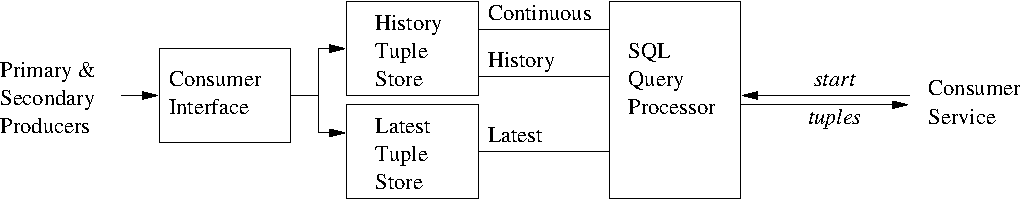
\includegraphics[width=160mm]{sp_detail}
\end{center}

The value of a Secondary Producer is that it creates real tables from
virtual ones, because it collects all tuples inserted into the virtual database
for any table it's republishing, into its own tuple stores. This means it can
act as an archiver for the tables, can answer queries involving joins between
them (even tables in different VDBs) because they're all in one database,
and can be used to reduce the load on other producers.

The Secondary Producer Service is responsible for authenticating all
users and services that connect to it, and for authorizing all
operations and all requests to access its tuple stores, as specified
in chapter \ref{sec:Security}.

\subsection{Interface}

\subsubsection{User Interface}

\begin{method}{createSecondaryProducer}
\inpar{xsd:boolean isHistory}{If history queries are supported}
\inpar{xsd:boolean isLatest}{If latest queries are supported}
\inpar{xsd:string type} {DATABASE or MEMORY}
\inpar{xsd:string logicalName}{The logical name should not be
be specified for type MEMORY. For type DATABASE it is optional.} 
\outhead{Tuple(1..1)}{}
\outpar{xsd:int connectionId}{connectionId of new Secondary Producer resource.} 
\desc Creates a new Secondary Producer resource and returns its endpoint. The
Secondary Producer is not added to a Registry until \textit{declareTable} is
called. The user cannot prevent Secondary Producers from supporting
continuous queries, but support for latest and/or history queries is optional.
Secondary Producers can use any type of storage, regardless of the query types
they support. Tuple stores can be made permanent by providing a
\textit{logical name} for the tuple store as described in
\ref{sec:SecondaryProducerTupleStores}.
The termination interval is described in \ref{sec:SecondaryProducerCreating}.
\end{method}

\begin{method}{declareTable}
\inpar{xsd:int connectionId}{Secondary Producer resource identifier.}
\inpar{xsd:string tableName}{VDBTable to register.}
\inpar{xsd:string predicate}{Producer's predicate.}
\inpar{xsd:int hrpSec}{History Retention Period in seconds.}
\OK
\desc
Adds a table to the list of tables republished by this producer, as described
in \ref{sec:SecondaryProducerDeclaring}. The table name must have an explicit
virtual database name prefix (separated from it by a dot).
The format of the
predicate is specified in \ref{sec:SQLPredicates}; by construction, a Secondary
Producer will republish \textit{all} tuples that match its predicate. The
retention period is described in \ref{sec:SecondaryProducerRemoving}.\\
\end{method}\par

\begin{method}{showSignOfLife}
\inpar{xsd:int connectionId}{Resource identifier.}
\OK
\desc Sends a sign-of-life request to a resource as a way to keep
the resource alive. Any other user operation on the resource will also serve
to keep it alive.
\end{method}

See also the common producer service operations:
getHistoryRetentionperiod~\ref{op:getHistoryRetentionPeriod}.

See also the common resource management service operations:
close~\ref{op:close} and destroy~\ref{op:destroy}.

See also the operations common to all services:
getProperty~\ref{op:getProperty}.

\subsubsection{System Interface}

\begin{method}{secondary}{addProducer}
\inpar{xsd:int connectionId}{Consumer resource identifier.}
\inpar{xsd:string url}{Producer URL.}
\inpar{xsd:int id}{Producer resource identifier.}
\inpar{xsd:string tableName}{Table name}
\inpar{xsd:string predicate}{Predicate}
\inpar{xsd:int hrpSec}{History Retention Period in seconds}
\inpar{xsd:boolean isHistory} {If producer supports history queries}
\inpar{xsd:boolean isLatest}{If producer supports latest queries}
\inpar{xsd:boolean isContinuous}{If producer supports continuous queries}
\inpar{xsd:boolean isStatic}{If producer supports static queries}
\inpar{xsd:boolean isSecondaryProducer}{If producer is secondary}
\inpar{xsd:string qosAttrib}{The QOS attribute - not used currently}
\OK
\desc Sent by a producer service to a continuous consumer or secondary producer
to notify it about an
addition to the list of relevant producers in the registry. Ignored if the
query is not currently executing. See the \textit{plan maintenance} section
(\ref{sec:ConsumerPlanMaintenance}) for how the consumer or secondary
producer should react to this.
\end{method}

\begin{method}{removeProducer}
\inpar{xsd:int connectionId}{Consumer resource identifier.}
\inpar{xsd:string url}{Producer URL.}
\inpar{xsd:int id}{Producer resource identifier.}
\OK
\end{method}

See  the common producer service operations:
start~\ref{op:start} and abort~\ref{op:producerabort}.

See the common resource management service operation:
ping~\ref{op:resourceping}.

\subsection{Details}
\subsubsection{Creating and destroying Secondary Producers}\label{sec:SecondaryProducerCreating}

A new Secondary Producer resource is created when a user calls the
\textit{createSecondaryProducer} operation and is destroyed when the user calls
the \textit{close} or \textit{destroy} operations. In addition,
if the service does not hear from the user for a period exceeding the
\textit{termination interval}, the service will initiate a \textit{close} operation
on the resource. A call to any user operation on the resource is sufficient
to keep it alive.

\subsubsection{Tuple stores}\label{sec:SecondaryProducerTupleStores}

These are exactly as in the Primary Producer Service (see
\ref{sec:PrimaryProducerTupleStores}) but System Administrators should
be even more wary of granting direct access to permanent tuple stores
maintained by Secondary Producers because Secondary Producers are granted
special access to the tuple stores of the producers from which they are
consuming, and those producers trust them to enforce the data access rules
of the VDB when republishing the data.

\subsubsection{Declaring tables (as a producer)}\label{sec:SecondaryProducerDeclaring}

The semantics of \textit{declareTable} are identical from the user's point of 
view to the Primary Producer, except that there is no Latest Retention Period 
to set. Internally, the service prepares the tuple stores then registers the 
Secondary Producer resource as a producer by calling 
\textit{registerProducerTable} and periodically calls this again to keep itself 
registered.

\subsubsection{Declaring tables (as a consumer)}\label{sec:ConsumerDeclaring}

Unlike a Primary Producer, the Secondary Producer must also act as a continuous
consumer for each declared table, by running a 
``SELECT * FROM \textit{tableName} WHERE \textit{predicate}'' query on the
virtual database. The procedure for identifying and notifying the producers
that will answer this query is exactly as in \ref{sec:ConsumerStarting} and
the list of producers is maintained as described in
\ref{sec:ConsumerPlanMaintenance}. A side effect of this is to register the
Secondary Producer resource as a \textit{secondary} consumer and keep it
registered. Flagging the resource as a secondary consumer simply allows
the mediator to ensure that it doesn't generate recursive query plans - in all
other respects, the mediator and the registry service treat the secondary
producer resource like any other continuous consumer and no further distinction
is made in this document. Likewise, the secondary producer presents the same
streaming interface to producers as described in
\ref{sec:ConsumerStreaming} for continuous consumers.

\subsubsection{Inserting tuples}\label{sec:SecondaryProducerInserting}
Tuples are inserted into a Secondary Producer by the service itself (by its 
streaming server). Users do not insert tuples into a Secondary Producer 
directly. Secondary Producers do not modify the tuples they store in any way.

\subsubsection{Removing tuples}\label{sec:SecondaryProducerRemoving}
The rules for History Retention Periods and Latest Retention Times in a
secondary producer are identical to a primary producer.

The \textit{close} call, however, is different from a primary producer. Since a
secondary producer must stop consuming immediately after a \textit{close}
request it must also stop servicing queries too, because it no longer holds a
complete set of tuples for the tables that it claims to republish.
Therefore \textit{close} means the same as \textit{destroy} in a secondary
producer.

\subsubsection{Processing queries}\label{sec:SecondaryProducerQueryProcessing}

Query processing in a Secondary Producer is identical to a Primary Producer
(see \ref{sec:PrimaryProducerQueryProcessing}).

\subsubsection{Stopping queries}\label{sec:SecondaryProducerStoppingQueries}

This is also identical to a Primary Producer
(see \ref{sec:PrimaryProducerStoppingQueries}).



\newpage
\section{On-demand Producer Service}\label{sec:OnDemandProducer}\index{on demand producer}
\subsection{Description}

On-demand Producer resources are created by the On-demand Producer Service
at the request of a user who wishes to make an external data store available
through a virtual database. They are registered in the same way as the other
producer types and their queries are parsed, validated and authorized like
queries to the other producer types, but they only support static queries,
are not used by Secondary Producers, have no internal tuple storage, and
have no concept of retention periods. As the picture below shows, queries are
simply handed off to a user-defined application (\textit{query handler}) that
is expected to process the query and return the resulting tuples on demand.

\begin{center}
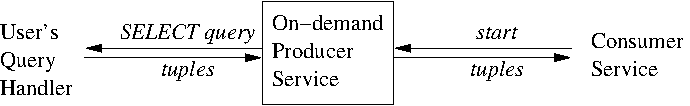
\includegraphics[width=110mm]{odp_detail}
\end{center}

The On-demand Producer Service is responsible for authenticating all users and
services that connect to it and for authorizing all operations and requests to
access its users' external data stores, as specified in chapter
\ref{sec:Security}.

\subsection{Interface}

\subsubsection{User Interface}

\begin{method}{createOnDemandProducer}
\inpar{xsd:string hostName}{Hostname of machine to which to connect to get data
to answer queries.}
\inpar{xsd:int port}{Port to which to connect to get data
to answer queries.}
\outhead{Tuple(1..1)}{}
\outpar{xsd:int connectionId}{connectionId of new On-demand Producer resource.} 
\desc
Creates a new On-demand Producer resource and returns its endpoint. The
On-demand Producer is not added to a Registry until \textit{declareTable} is
called. On-demand producers have no tuple stores and only support static
queries.
\end{method}


\begin{method}{declareTable}
\inpar{xsd:int connectionId}{On-demand Producer resource identifier.}
\inpar{xsd:string tableName}{VDBTable to register.}
\inpar{xsd:string predicate}{Producer's predicate.}
\OK
\desc
Adds a table to the list of tables for which this producer will return tuples,
as described in \ref{sec:OnDemandProducerDeclaring}.
The table name must have an explicit virtual database name prefix (separated
from it by a dot). The format of the predicate is specified
in \ref{sec:SQLPredicates}; all returned tuples must match this predicate or
they will be rejected by the producer. 
\end{method}

See also the common producer service operations:
getHistoryRetentionperiod~\ref{op:getHistoryRetentionPeriod}.

See also the common resource management service operations:
close~\ref{op:close} and
destroy~\ref{op:destroy}.

See also the operations common to all services:
getProperty~\ref{op:getProperty}.

\subsubsection{System Interface}

See  the common producer service operations:
start~\ref{op:start} and abort~\ref{op:producerabort}.

See the common resource management service operation:
ping~\ref{op:resourceping}.

\subsection{Details}
\subsubsection{Creating and destroying On-demand Producers}\label{sec:OnDemandProducerCreating}

A new on-demand producer resource is created when a user calls the
\textit{createOnDemandProducer} operation and is destroyed when the
user calls the \textit{close} or \textit{destroy} operations. In
addition, if the service does not hear from the user for a period
exceeding the \textit{termination interval}, the service will initiate
a \textit{close} operation on the resource. A call to any user
operation on the resource is sufficient to keep it alive.

\subsubsection{The query handler}

The on-demand producer connects to the specifed hostname and port via an SSL
socket connection to answer user queries. R-GMA
expects the query handler application to be listening for queries
throughout the lifetime of the on-demand producer resource.

\subsubsection{Declaring tables}\label{sec:OnDemandProducerDeclaring}

On-demand producers must register any tables for which they will
answer queries by calling \textit{declareTable}. The On-demand
Producer Service registers the producer as a publisher for that table
by calling the registry's \textit{registerProducerTable} operation and
will periodically re-send the \textit{registerProducerTable} to the
registry on the user's behalf, to maintain the producer's entries in
the registry throughout its lifetime. The user can declare more than
one table in a single producer, and these can even be in different
virtual databases. Whether or not ``join'' queries can be processed
depends only on the capabilities of the query handler that answers the
producer's queries.

\subsubsection{Processing Queries}\label{sec:OnDemandProducerQueryProcessing}

Consumer Services send a \textit{start} message to an On-demand
Producer to request it to execute a query and start streaming the
resulting tuples back to the consumer service. The query is forwarded
to the registered query handler for processing (see below for the protocol),
and the tuples (if any)
returned by the query handler are streamed by the On-demand Producer service
back to the consumer's streaming server, exactly as in a one-time query to
any other type of producer (see \ref{sec:ConsumerStreaming}). A query may be
stopped by the consumer service by calling \textit{abort}. Queries
will also be automatically aborted by the On-demand Producer Service
if they run for more than the \textit{timeout} specified in the call
to \textit{start}.

The On-demand producer service will append the standard metadata columns
(see \ref{sec:PrimaryProducerInserting}) to each tuple for
consistency with the table definition in the schema, before streaming
them back to the consumer service, but the columns will all be populated
with NULLs.

See section
\ref{sec:SQLCharacterSets} for information about the character sets used in
R-GMA (this will affect both the SQL query sent to the query handler, and its
response).

\subsubsection{Query handler protocol}

The On-demand Producer service contacts the query handler by opening a TCP
connection on the host
and port specified in the URI and writing the SQL SELECT query and the maximum
number of tuples it will allow in a result set, to the port. The two parameters
are separated by a semi-colon and the request is terminated by a CR-NL end of 
line marker. The query handler must respond by sending a series of result sets
(chunks) each containing no more than the requested number of tuples, or it must
return an exception. The query handler should mark the end of the response by
shutting the TCP connection.

The result sets and exceptions returned by the query handler are XML fragments,
each containing a single XMLResultSet or XMLException. The XMLResultSet looks
like this:

\begin{verbatim}
<?xml version="1.0" encoding="UTF-8" standalone="no"?>
  <XMLResultSet endOfResults="true">
    <columnMetaData>
      <name>column-name</name>
      <type>NNN</type>
      <table>table-name</table>
    </columnMetaData>
    <row>
      <col>column-value</col>
      <col isNull="true"/>
    </row>
  </XMLResultSet>
\end{verbatim}
                                                                                
where \textit{columnMetaData} and \textit{col} are repeated for each
column, and \textit{row} is repeated for each row. The valid values
for \textit{type} are 4 (INTEGER), 7 (REAL), 8 (DOUBLE PRECISION), 91
(DATE), 92 (TIME), 93 (TIMESTAMP), 1 (CHAR) and 12 (VARCHAR). The
\textit{endOfResults} and \textit{isNull} flags both default to \textit{false} if
omitted. The \textit{XMLResultSet} element is allowed to be entirely
empty.  The last result set must contain an \textit{endOfResults} flag
set to \textit{true} (even if it is empty).

The XMLException looks like this:

\begin{verbatim}
<?xml version="1.0" encoding="UTF-8" standalone="no"?>
  <XMLException>
    <message>message-string</message>
  <XMLException>
\end{verbatim}

The On-demand producer service will shut the TCP connection if the query
handler exceeds the tuple limit in a single result set (chunk), or
it receives an \textit{abort} request, or if some other error occurs. The
query handler must ensure that the result of a query does not change during
the time it takes to deliver all of the tuples to the on-demand producer
service.

\subsection{Error Handling}

The default handling for all errors is to stop processing, make the resource
stable if possible and notify the user
(see section \ref{sec:BackgroundErrorReporting}).

\newpage
\section{Producer Services}

These extend the ResourceManagementService. Their primary function is to manage
the  producer resources. 

\subsection{Primary Producer Service}
\label{sec:primaryProducerService}
\index{Service!Primary Producer}

\subsection{Secondary Producer Service}
\label{sec:secondaryProducerService}
\index{Service!Secondary Producer}

\subsection{On-demand Producer Service}
\label{sec:onDemandProducerService}
\index{Service!On-demand Producer}





\newpage
\section{Consumer Service}
\label{sec:consumerService}
\index{Service!Consumer}

Package: \texttt{org.glite.rgma.server.services.consumer}


This extends the ResourceManagementService. Its primary function is to manage
the consumer resources. The consumer resource 
extends the \texttt{Resource} described in
Section~\ref{sec:Resource} in addition to the states defined by a
resource it has a mode which must be one of:

\begin{description}

\item[NEW] Not yet started

\item[STARTED] Start has been called

\item[RUNNING] Plan has been generated and producers started

\item[FINISHED] Query completed

\item[ABORTED] Query aborted

\end{description}

The transition from \texttt{STARTED} to \texttt{RUNNING} is made by the 
GetPlans task for a normal start call and is set directly within a start call 
for a directed query. The transition from \texttt{RUNNING} to \texttt{FINISHED} 
is triggered by the \texttt{pop()} call.

The ConsumerResource deals with plans from the mediator. These all require calls
to the registry and so make use of the task queue. For any resource only one plan
related task should be queued at any one time so a single variable is used to
keep track of these tasks.

Each Consumer Resource has a Tuple Queue.  The Tuple Queue is entirely private 
to the Consumer Resource - the Streaming Receiver Thread (see
Sec.\ref{sec:queryAnsweringSubsystem} calls the resource's 
\texttt{insert()} method (defined by its Streaming Sink Interface) to add 
tuples, and the Consumer Service calls the resource's \texttt{pop()} method to 
remove them. Although the Consumer Service will authorize each call to the pop 
operation itself, access to the data in the Tuple Queue requires no further 
authorization. There is no timeout or cleanup of tuples in the Tuple Queue - 
the termination interval of the Consumer Resource itself is sufficient. The 
Tuple Queue holds a number of tuples in memory. If the maximum tuples in memory 
is exceeded, a group of tuples is taken off the queue and stored in a DB table 
with a unique incrementing ID to preserve the order. A ``read'' and ``write'' 
pointer to the RB table is kept in memory so that a group of tuples can be 
popped with a single query. Tuples are taken first from the data base table and 
then from memory to preserve the queue ordering.

If the tuple queue fills up, the consumer's query is aborted. It does this by
calling the abort(RGMAException) on the consumer so that the exception can
be stored and returned at the next pop() call.

\newpage
\section{Resource Management Operations}\label{sec:Resource}\index{resource 
management operations}

Operations defined here are are common to all resource management operations - i.e.
producers and consumers.

\subsection{Interface}

\subsubsection{User Interface}

\begin{method}{close}
\inpar{xsd:int connectionId}{Resource identifier.}
\OK
\desc Schedules a resource for destruction after the resource has completed its work.
\end{method}

\begin{method}{destroy}
\inpar{xsd:int connectionId}{Primary Producer resource identifier.}
\OK
\desc 
Destroys a Primary Producer without any special \textit{close} processing.
\end{method}


\subsubsection{System Interface}

\begin{method}[resource]{ping}
\inpar{xsd:int connectionId}{Resource identifier.}
\OK
\desc
Checks if a resource is still alive (and throws an exception if it is not).
Has no side-effects on the resource. 
\end{method}

\newpage
\section{Registry Service}\label{sec:Registry}\index{registry}
\subsection{Description}

There is exactly one registry per virtual database. It holds the
details of all producers that are publishing to tables in the virtual
database, and it also holds the details of continuous consumers who wish to be
notified of changes to the list of producers. For reasons of resilience and
scalability, multiple replicas of the registry can be created for each virtual
database. Each replica exists as a Registry Instance in a Registry Service and
is created by the service at the request of a user. A single Registry
Service can host replicas from multiple virtual databases. The Registry Service
also handles queries for registries that it is not hosting, by locating
another Registry Service that is hosting a working replica of the requested
registry and forwarding the query there. In this way, users, producer services
and consumer services only ever need to contact their local Registry Service
directly.

The Registry Service is responsible for authenticating all users and services
that connect to it, and for authorizing all operations and all requests to
access the registries it is hosting, as specified in chapter \ref{sec:Security}.

\subsection{Interface}

\subsubsection{User Interface}

\begin{method}{getAllProducersForTable}
\inpar{xsd:string vdbName}{Virtual database name.}
\inpar{xsd:boolean canForward}{True if query can be forwarded.}
\inpar{xsd:string tableName}{Table name.}
\outhead{Tuple(0..*)}{}
\outpar{xsd:string url}{Producer URL}
\outpar{xsd:int connectionId}{Producer resource ID.}
\outpar{xsd:boolean isSecondaryProducer}{If producer is secondary.}     
\outpar{xsd:boolean isContinuous}{If producer supports continuous queries.}  
\outpar{xsd:boolean isStatic}{If producer supports static queries.}     	
\outpar{xsd:boolean isHistory}{If producer supports history queries.}  
\outpar{xsd:boolean isLatest}{If producer supports latest queries.}  
\outpar{xsd:string predicate}{Predicate associated with the producer.}
\outpar{xsd:int hrpSec}{History Retention Period in seconds} 	
\desc Returns an unmediated list of all producers registered for the specified
tables, with their connection details and producer types (used by the R-GMA
Browser). Processed locally if possible (see \ref {sec:RegistryForwarding}).\\
\end{method}

See also the operations common to all services: getProperty~\ref{op:getProperty}.


\subsubsection{System Interface}


getURL(), getResourceID(), isSecondary(), isContinuous(), isStatic(),
isHistory(),  isLatest(), getPredicate(),getHistoryRetentionPeriod(), getVdbName(), getTableName()
				
\begin{method}{getMatchingProducersForTables}
\inpar{xsd:string vdbName}{Virtual database name.}
\inpar{xsd:boolean canForward}{True if query can be forwarded.}
\inpar{xsd:string(1..*) tables}{Table name}
\inpar{xsd:string predicate}{Predicate associated with the
consumer.}       
\inpar{xsd:string queryType}{Consumer's Query type.}
\inpar{xsd:int(0..1) timeIntervalSec}{Time interval to look back into the past
for matching tuples.}
\inpar{xsd:boolean isSecondaryConsumer}{True for secondary consumer (i.e. consumer part of a secondary
producer). Only specified if queryType is continuous.}
\inpar{xsd:string url}{URL of consumer. Only specified if queryType is
continuous.}
\inpar{xsd:int resourceId}{Resource id of consumer. Only specified if queryType
is continuous.}
\inpar{xsd:int terminationIntervalSec}{Consumer's termination interval in seconds.}
\outhead{Tuple(0..*)}{}
\outpar{xsd:string url}{Producer URL}
\outpar{xsd:int connectionId}{Producer resource ID.}
\outpar{xsd:boolean isSecondaryProducer}{If producer is secondary.}     
\outpar{xsd:boolean isContinuous}{If producer supports continuous queries.}  
\outpar{xsd:boolean isStatic}{If producer supports static queries.}     	
\outpar{xsd:boolean isHistory}{If producer supports history queries.}  
\outpar{xsd:boolean isLatest}{If producer supports latest queries.}  
\outpar{xsd:string predicate}{Predicate associated with the producer.}
\outpar{xsd:int hrpSec}{History Retention Period in seconds}
\outpar{xsd:string tableName}{Table name without VDB prefix.}
\outpar{xsd:string vdbName}{Virtual database name.}
\desc Returns a list of all producer-table entries from the registry that match
the Consumer's query predicate, for any of the listed tables. This operation is
used by the mediator in the consumer service. Continuous
consumers are also registered (or updated if they are already registered)
by this call so the registry can pass their details to any new, relevant
producers. See
\ref{sec:RegistryRegistering} for a description of the termination interval.
The last three parameters: \textit{isSecondary}, \textit{consumer} and
\textit{terminationIntervalSec}
are only present for continuous consumers.
Processed locally if possible (see \ref {sec:RegistryForwarding}).
\end{method}

\begin{method}{registerProducerTable}
\inpar{xsd:string vdbName}{Virtual database name.}
\inpar{xsd:boolean canForward}{True if query can be forwarded.}
\inpar{xsd:string url}{Producer URL}
\inpar{xsd:int id}{Producer resource ID.}
\inpar{xsd:string tableName}{Table name.}
\inpar{xsd:string predicate}{Producer's predicate.}
\inpar{xsd:boolean isContinuous}{If producer supports continuous queries.}  
\inpar{xsd:boolean isHistory}{If producer supports history queries.}  
\inpar{xsd:boolean isLatest}{If producer supports latest queries.}  
\inpar{xsd:boolean isStatic}{If producer supports static queries.}
\inpar{xsd:boolean isSecondaryProducer}{If producer is secondary.}
\inpar{xsd:int hrpSec}{Table's History Retention Period in seconds.}
\inpar{xsd:int terminationIntervalSec}{Producer's termination interval in
seconds.}
\outhead{Tuple(0..*)}{}
\outpar{xsd:string url}{Consumer URL}
\outpar{xsd:int id}{Consumer resource ID.}
\desc Adds an entry to the Registry for a producer containing the details passed
to this operation or updates them if it is already registered. The producer
service
will already have validated the predicate before calling this operation.
If the new producer supports continuous queries and there are any registered
continuous consumers to which this producer is relevant (by comparison of
their predicates), then this call returns a list so the producer can
send an \textit{addProducer} notification to each of them (the list will be
empty for non-continuous producers).
The \textit{retentionPeriod} should reflect the actual history
available from the producer (which may be very short initially) and should
be updated in subsequent calls to this operation. See
\ref{sec:RegistryRegistering} for a description of the
termination interval.
Processed locally if possible (see \ref {sec:RegistryForwarding}).
\end{method}

\begin{method}{unregisterContinuousConsumer}
\inpar{xsd:string vdbName}{Virtual database name.}
\inpar{xsd:boolean canForward}{True if query can be forwarded.}
\inpar{xsd:string url}{Consumer URL}
\inpar{xsd:int id}{Consumer ID.}
\desc Removes a Continuous consumer's entry from the Registry. The Consumer
Service is expected to notify all producers to which the consumer has subscribed that
it is closing - the Registry does not do this.
Processed locally if possible (see \ref {sec:RegistryForwarding}).
\end{method}

\begin{method}{unregisterProducerTable}
\inpar{xsd:string vdbName}{Virtual database name.}
\inpar{xsd:boolean canForward}{True if query can be forwarded.}
\inpar{xsd:string tableName}{Table name.}
\inpar{xsd:string url}{Producer's URL}
\inpar{xsd:int id}{Producer's ID.}
\desc Removes a producer's entry for a particular table from the Registry.
Processed locally if possible (see \ref {sec:RegistryForwarding}).
\end{method}

\begin{method}{addReplica}
\inpar{xsd:string replica}{String with replication message for a vdb.}
\desc Applies updates to the Registry with data from another replica. See section
\ref{sec:RegistryReplication} for details. Always processed locally.
\end{method}

\begin{method}[registry]{ping}
\inpar{xsd:int vdbName}{Virtual database name}
\OK
\desc
Checks if a registry instance is still alive (and throws an exception
if it is not). Used by the Registry Service to locate the ``closest''
working replica for a particular virtual database. Has no side-effects
on the registry instance.  Always processed locally.
\end{method}


\subsection{Details}
\subsubsection{Registering and unregistering resources}\label{sec:RegistryRegistering}

Resources are registered when a service calls the
\textit{registerProducerTable} and \textit{getMatchingProducersForTables}
operations, and are unregistered when a service calls the
\textit{unregisterProducerTable} or
\textit{unregisterContinuousConsumer} operations. The registration calls must
be repeated periodically with the interval between calls not exceeding the
termination interval, otherwise the registry will automatically unregister the
resource. If the re-registration arrives late, it will simply put the entry
back as if it was a new entry. The registry instance which hosts the replica
notes the updates it receives and uses these to generate an \textit{addReplica}
call to send updates to all other registries it knows about.

\subsubsection{Forwarding operations}\label{sec:RegistryForwarding}\index{registry fowarding}

Most registry operations specify the name of the virtual database for
which they are intended. If the Registry Service is hosting a registry
replica for that virtual database, it will process the operation
locally. If it is not, it will attempt to locate another Registry
Service that is hosting a replica, then check that the replica is
still working (trying a different service if it is not), before
forwarding the operation to that service and returning the
results. This forwarding can be prevented by setting the
\textit{canForward} to \textit{false} in those operations that support
it: this is meant for use by Registry Services only, to prevent an
operation from being forwarded more than once, and is hidden by the
User APIs. How the Registry Service obtains URLs of other Registry
Services and lists of the virtual databases for which they are hosting
replicas, is described in \ref{sec:BackgroundBootstrapping}. The rules
about when to switch from one replica to another are given in the next
section.

\subsubsection{Replication}\label{sec:RegistryReplication}\index{registry replication}

When a Registry Service receives a request intended for a replica in a
virtual database that it has not contacted before, it chooses the
``best'' replica in some implementation-defined way that is likely to
be based on round-trip times for calls to \textit{ping} on each
replica. It then uses this replica for all subsequent requests for
that virtual database, until it is forced to switch either because the
replica fails, or it discovers that new replicas have been added
(e.g. for load balancing).

The Registry Service runs a replication cycle, with a
site-configurable frequency, for each replica that it is hosting
locally. At each cycle, it sends updates made to the replica to all
other replicas in the same virtual database, by calling
\textit{addReplica}. As far as possible, change-only updates are used
to minimize the size of the replication messages.

A new registry replica will be empty initially. A restarted replica
will reload any entries it had before. In both cases, the replica will
wait until one full replication cycle has been attempted before it
will start servicing queries (regardless of whether or not it has
heard from all other replicas).

Since replicas will become inconsistent with each other between
replication cycles, all R-GMA services must tolerate a registry
informing them about producer and consumer resources that no longer
exist, or failing to inform them about ones about which it does not
yet know.

\subsubsection{Registry Database}\index{registry database}

The Registry maintains two lists, one containing an entry for each table of
each producer publishing to the virtual database, and one containing an entry
for each continuous consumer querying the virtual database. How these are
stored is implementation dependent, but they're likely to be database tables.
It is a requirement that their contents can survive the Registry
Service being restarted. The lists need to contain just sufficient details
for the Registry Service operations to be supported.

\newpage
\section{Schema Service}\label{sec:Schema}\index{schema}
\subsection{Description}

There is exactly one schema per virtual database. It holds the names and 
definitions of all of the tables in the virtual database, and their 
authorization rules. Each server holds a copy of the schema for each virtual 
database it supports. Unlike the registry, requests are not forwarded as each 
server has its own copy. As part of the R-GMA configuration one schema should 
be designated as master for each virtual database. Each server is configured 
with a file for each virtual data base it supports identifying the master 
schema. The slaves poll the master periodically to obtain updates.

The Schema Service is responsible for authenticating all clients and
services that connect to it, and for authorizing all operations and
all requests to access the schemas it is hosting, as specified in
chapter \ref{sec:Security}.

Note that all operations that change the schema return a boolean flag
\textit{changed} which is true if the state of the schema has (or may have been
changed). This is for internal use as changes are made first to the master
schema and then if changes have been made the local schema is updated from the
master. The flag is not exposed by the user API.

\subsection{Interface}

\subsubsection{User Interface}
The following operations are available to client applications.

\begin{method}{createTable}\index{create table}
\inpar{xsd:string vdbName}{Virtual database name.}
\inpar{xsd:string createTableStatement}{SQL CREATE TABLE statement.}
\inpar{rgma:StringList tableAuthz}{Table authorization rules.}
\outhead{Tuple}{}
\outpar{xsd:boolean changed}{True if any changes made.}
\desc Adds a new table definition to the schema of the requested virtual database.
Rules for naming tables and columns, supported column types and the format of
the CREATE TABLE statement are all specified in chapter \ref{sec:SQL}. The
authorization rules are described in chapter \ref{sec:Security}. 
\end{method}

\begin{method}{dropTable}\index{drop table}
\inpar{xsd:string vdbName}{Virtual database name.}
\inpar{xsd:string tableName}{Table name.}
\outhead{Tuple}{}
\outpar{xsd:boolean changed}{True if any changes made.}
\desc Drops a table from the schema of the requested virtual database.
\end{method}

\begin{method}{alter}\index{alter}
\inpar{xsd:string vdbName}{Virtual database name.}
\inpar{xsd:string torv}{TABLE or VIEW.}
\inpar{xsd:string tableName}{Table name.}
\inpar{xsd:string action}{ADD, DROP or MODIFY.}
\inpar{xsd:string name}{Column name.}
\inpar{xsd:string type (0..1)}{Column type.}
\outhead{Tuple}{}
\outpar{xsd:boolean changed}{True if any changes made.}
\desc Alter a table defintion. \textit{add} and \textit{drop} are permitted
for a table or view and \textit{modify} to a table. The column type must be
specified for \textit{add} and  \textit{modify} on a table and in no other case.
\end{method}

\begin{method}{createIndex}
\inpar{xsd:string vdbName}{Virtual database name.}
\inpar{xsd:string createIndexStatement}{SQL CREATE INDEX statement.}
\outhead{Tuple}{}
\outpar{xsd:boolean changed}{True if any changes made.}
\desc Adds a new index definition for an existing table in a schema of the requested
virtual database. The format of the CREATE INDEX statement is specified in
\ref{sec:SQLCreateIndex}. Indexes cannot be defined for views. 
\end{method}

\begin{method}{dropIndex}
\inpar{xsd:string vdbName}{Virtual database name.}
\inpar{xsd:string indexName}{Index name.}
\outhead{Tuple}{}
\outpar{xsd:boolean changed}{True if any changes made.}
\desc Drops an index from the schema of the requested virtual database.
\end{method}

\begin{method}{createView}
\inpar{xsd:string vdbName}{Virtual database name.}
\inpar{xsd:string createViewStatement}{SQL CREATE VIEW statement.}
\inpar{rgma:StringList viewAuthz}{View authorization rules.}
\outhead{Tuple}{}
\outpar{xsd:boolean changed}{True if any changes made.}
\desc Adds a new view definition on an existing table in a schema of the requested
virtual database. Views are described in \ref{sec:SecurityViews} and the format
of the CREATE VIEW statement is specified in \ref{sec:SQLCreateView}. 
\end{method}

\begin{method}{dropView}
\inpar{xsd:string vdbName}{Virtual database name.}
\inpar{xsd:string viewName}{View name.}
\outhead{Tuple}{}
\outpar{xsd:boolean changed}{True if any changes made.}
\desc Drops a view from the schema of the requested virtual database.
\end{method}

\begin{method}{getAllTables}
\inpar{xsd:string vdbName}{Virtual database name.}
\outhead{Tuple (0..*)}{}
\outpar{xsd:string tableName}{Table or view name.}
\desc Returns a list of all table and view names in the schema of the requested
virtual database (no distinction is made between tables and views).
\end{method}

\begin{method}{getTableDefinition}
\inpar{xsd:string vdbName}{Virtual database name.}
\inpar{xsd:string tableName}{Table or view name.}
\outhead{Tuple (0..*)}{}
\outpar{xsd:string tableName}{Table or view name.}
\outpar{xsd:string columnName}{Name of column}
\outpar{xsd:string columnType}{Type of column - e.g. REAL or INTEGER}
\outpar{xsd:integer columnSize}{Size of column}
\outpar{xsd:boolean columnIsNotNull}{{If column is NOT NULL}}
\outpar{xsd:boolean columnIsPrimaryKey}{If column is PRIMARY KEY}
\outpar{xsd:string viewFor}{}
\desc Returns a table's column definitions from the schema of the requested virtual
database (used by the R-GMA Browser). If \textit{tableName} is a view, only
returns details of those columns in the view.
\end{method}

\begin{method}{getTableIndexes}
\inpar{xsd:string vdbName}{Virtual database name.}
\inpar{xsd:string tableName}{Table name.}
\outhead{Tuple (0..*)}{}
\outpar{xsd:string indexName}{Table or index.}
\outpar{xsd:string columnName}{Name of column}
\desc Returns a list of the indexes associated with a table (indexes cannot be
associated with a view).
\end{method}

\begin{method}{setAuthorizationRules}
\inpar{xsd:string vdbName}{Virtual database name.}
\inpar{xsd:string tableName}{Table or view name.}
\inpar{rgma:StringList tableAuthz}{Table authorization rules.}
\outhead{Tuple}{}
\outpar{xsd:boolean changed}{True if any changes made.}
\desc Replaces a table's or view's read/write authorization rules. The authorization
rules are described in chapter \ref{sec:Security}. 
\end{method}

\begin{method}{getAuthorizationRules}
\inpar{xsd:string vdbName}{Virtual database name.}
\inpar{xsd:string tableName}{Table or view name.}
\outhead{Tuple (0..*)}{}
\outpar{xsd:string authzRule}{Authorization rule.}
\desc Returns the read/write authorization rules associated with a table or view.
Authorization rules are described in chapter \ref{sec:Security}.
\end{method}

See also the operations common to all services:
getProperty~\ref{op:getProperty}.

\subsubsection{System Interface}
The following operations are available to other R-GMA services only.

\begin{method}{getTableTimestamp}
\inpar{xsd:string vdbName}{Virtual database name.}
\inpar{xsd:string tableName}{Table name.}
\outhead{Tuple}{}
\outpar{xsd:long timeStamp}{TimeStamp in ms since 1970.}
\desc Returns timestamp when table definition was last modified.
\end{method}


\begin{method}{getSchemaUpdates}
\inpar{xsd:string vdbName}{Virtual database name.}
\inpar{xsd:long timeStamp}{TimeStamp in ms since 1970.}
\outpar{xsd:string updates}{Table details.}
\desc Returns full information for each table that has changed since the
specified timestamp - which may be zero.
\end{method}
                                                                                
\subsubsection{Replication}\label{sec:SchemaReplication}
Periodically each slave schema sends a request to the master for updates.

\subsubsection{Schema Database}\index{schema database}

The Schema maintains lists of the definitions of all tables in the virtual
database, and their access permissions. How these are stored is implementation
dependent, but they're likely to be database tables. It is a requirement that
their contents can survive the Schema Service being restarted. The lists need
to contain just sufficient details for the Schema Service operations to be
supported.

\newpage
\section{Service Operations}\label{sec:Service}\index{service operations}

Operations defined here are are common to all services.

\subsection{Interface}

\subsubsection{User Interface}

\begin{method}{getProperty}
\inpar{xsd:string name}{Property name.}
\inpar{xsd:string(0..1) parameter }{Property parameter.}
\outhead{xml:Any}{Property value.}
\desc Returns the current value of the requested service property. The appropriate
contents of \textit{parameter} depend on the property name. The list of
service properties is extensible and subject to change without warning.
\end{method}

\subsubsection{System Interface}

\newpage
\section{RGMAService Operations}\label{sec:Producer}\index{producer}

The RGMAService is for functions not directly related to producers, consumers,
registry or schema.

\subsection{Interface}

\subsubsection{User Interface}

\begin{method}{listTupleStores}
\outhead{Tuple(0..*)}{}
\outpar{xsd:string logicalName}{Logical name of tuple store.}
\outpar{xsd:boolean isHistory}{If logical name is associated with a history store.} 
\outpar{xsd:boolean isLatest}{If logical name is associated with a latest store.}
\desc Returns a list of all of the permanent tuple stores. A logical name may be associated with both history and latest 
stores. Only the user's own tuple 
stores are listed.
\end{method}

\begin{method}{dropTupleStore}
\inpar{xsd:string logicalName}{Logical name of tuple store.}
\OK
\desc Permanently deletes a permanent tuple store, provided it is not currently being
used by a producer. Only the user's
own tuple stores can be dropped.
\end{method}

\begin{method}{getVersion}
\outhead{Tuple}{}
\outpar{xsd:string version}{Service version.}
\desc Returns the version number of the services.
\end{method}

\begin{method}{getTerminationInterval}
\outhead{Tuple)}{}
\outpar{xsd:int terminationIntervalSec}{Termination interval in seconds.}
\desc Returns the current termination interval defined by the services.
\end{method}

\newpage
\section{Security}\label{sec:Security}\index{security}

\subsection{Introduction}

In a secure installation, R-GMA services are responsible for ensuring
the integrity and confidentiality of the virtual databases and all
user data held within the service infrastructure.  This chapter
specifies the security mechanisms used by the services to meet this
responsibility. Sites can opt to run their services with these
security mechanisms turned off, but other R-GMA services running
securely will not communicate with them.

\subsection{Risks to services and data}

The integrity of a virtual database is compromised if a person
maliciously modifies data or causes operations to execute incorrectly
so that the virtual database reaches an invalid state or returns
invalid results. This can be achieved either by direct attacks on the
service infrastructure or by abusing the operations provided by
services.

The integrity and confidentiality of user data are compromised if a
person can read or modify the data without the owner's consent. User
data in R-GMA does not just include tuples, but also query strings
(because predicates may contain user data), resource connection
details (because these could be used to launch attacks), user
identification details stored for security purposes and user names and
passwords for external data stores.  Data integrity and
confidentiality can be compromised by a malicious person making direct
attacks on the service infrastructure or abusing the operations
provided by services. They can also be compromised by the failure of a
service implementation to properly enforce data access rules.

\subsection{Securing services and data}

The service infrastructure consists of the underlying operating
system, the servlet container, external
storage used by the services (e.g. databases, configuration files, log
files), connections between services and external storage (e.g. JDBC
links), and network connections to services. With the exception of the
network connections, it is beyond the scope of this specification to
say how these can be made secure, but it is mandatory for all R-GMA
service implementations to address the security of each of these
components.

How R-GMA services secure network transfers against interception and
modification, how they control connections to services and how they
control execute access to operations and read and write access to data
stores, are all covered in the remainder of this chapter.

\subsection{Securing network transers}

All user-to-service and service-to-service connections (including
streaming) in a secure R-GMA installation use SSL to encrypt the data
as it travels over the network. Data is \textit{not} encrypted by
R-GMA within its services. If users don't trust the security of
R-GMA's services, they must encrypt the data themselves before sending
it to R-GMA.
                                                                               

\subsection{Authentication}\index{authentication}

R-GMA services must immediately terminate a user's or other service's
attempt to connect to them if their identity cannot be
authenticated. If a user chooses to use one of the R-GMA APIs, the API
will likewise abandon a connection immediately if it cannot
authenticate the service to which it is connecting (this is
\textit{mutual authentication}). The APIs return an appropriate
RGMASecurityException in response to authentication failures.

Mutual authentication is based on an exchange of encrypted messages.
Each party's identity is proved by their possession of a private key
corresponding to the public key embedded in a digital certificate
signed by a certificate authority recognised by the other party.  Currently
R-GMA services accept only X509 format certificates (including proxy certificates generated by
grid-proxy-init or voms-proxy-init).

The mechanism used for authentication and for managing Certificate
Authority (CA) certificates and their supporting files (revocation
lists, signing policies, etc) is implementation-dependent.

\subsection{Authorization}\index{authorization}

\subsubsection{Credentials}\index{credentials}

R-GMA services permit or deny access to resources (in the general
sense) to a user or another service, on the basis of
\textit{credentials} held by that user or service. Credentials are
extracted from the certificate used for authentication in some
implementation-defined way. Each credential has a name such as the
{Distinguished Name} (DN) credential found in all
certificates\footnote{The DN of host certificates contains the host
name.}.  The credentials found in the \textit{VOMS proxy certificates}
used by all EGEE services are:

\begin{itemize}
\item Membership of virtual organizations (VO);
\item Membership of groups within a virtual organization (GROUP);
\item Roles held within a virtual organization (ROLE);
\end{itemize}

and some, such as GROUP, may take more than one value.  All
authorization rules are defined in terms of combinations of zero or
more credentials, and whilst R-GMA service implementations are obliged
to support VOMS credentials, they will actually work with any type of
credential.

\subsubsection{Ownership}\index{ownership}

The servers on which R-GMA services run are owned by individual
sites\index{site}, so it is they who decide whether or not to run the
services. 

Each virtual database has an owner (typically a VO) and registry 
instances and the master schema are hosted by sites by mutual agreement with the
virtual database owner. The virtual database owner owns the registry and schema instances and
decides who can read or modify them, but they have to trust the individual
sites to implement their policy, and the sites retain overall control.

Virtual database owners control who can create, read or modify information
the schema and who can read tuples from their virtual database and who can
publish tuples to it, because they own the schema and the data access rules are
defined there. Anybody permitted to write to a table defintion in the
schema can also control who can read or write to that table within the virtual
database.

\subsubsection{Authorization points}

Access to the tuples in the tuple stores is authorized using \textit{read} and 
\textit{write} rules set for each table and view in the schema. The rule-based 
mechanisms are described below.

Access to the schema information is controlled by rules stored as part of the
VDB in addition to rules stored with a table defintion in the schema.

\subsubsection{Restricting access to columns (views)}\label{sec:SecurityViews}\index{view}

Views are defined in the schema as a subset of the columns of a table
(the \textit{base table} of the view), created using the Schema
service's \textit{createView} operation (see
\ref{sec:SQLCreateView}). Users can query views just as they would
real tables, but they are read-only, so producers cannot publish to
them, and they do not appear in the registry. Their purpose is to
limit access to only certain columns of the base table: tuples read
from a view are actually read from the base table, but the query is
only allowed to include columns that form part of the
view. Authorization rules for row access to views are defined exactly
as for tables (see the next section) and completely replace the rules
on the base table.

\subsubsection{Authorizing read/write access to rows in tables or views}

All consumers (including those used by Secondary Producers) require read
authorization to read tuples from views or tables in the virtual database and
all producers (Primary, Secondary and On-demand) require write authorization
to publish tuples into tables in the virtual database.

These authorization rules are defined in the schema and the virtual database
owner decides who can change authorization rules in the schema by authorizing
the change operation as described above; the user who creates the table or view
sets the initial rules.

The producer services are responsible for enforcing the rules. In a Primary
Producer service, the write rules are applied in calls to \textit{insert} and
\textit{insertList}, and the read rules are applied in calls to \textit{start}.
In a Secondary Producer service, the write rules are ignored but the read rules
are applied as in a Primary Producer service. In an On-demand Producer service,
the write rules, followed by the read rules, are both applied in calls to
\textit{start}. In all cases, the producer services must
notice changes to the data access rules
and apply the changes to any tuples subsequently sent to a consumer service.
Note that enforcing read rules in the producer services requires the consumer
services to be able to prove that they are acting on behalf of the user or
service to which read access is being granted (this requires \textit{delegation}
of credentials).

The default rule is that no user is permitted any access to the table or view.
Rules are added to grant access only (not to deny it) and they are cumulative.
Read and write rules are formatted identically and have
the form ``\textit{predicate : credentials : action}'', where the three
clauses are defined as follows:

\begin{description}

\item[predicate]
Defines the subset of rows of the table or view to which this rule grants
access. It is an SQL WHERE clause that compares the values in specified
columns with constants, other columns or credential parameters (credential
name in square brackets, such as [DN]) that are replaced by the corresponding
credentials (or set of credentials) extracted from the user's certificate when
the rule is evaluated. The predicate expression is restricted to the following
operators: AND, OR, NOT, IN, \(=\), LIKE, \(<>\), \(<\), \(>\) and IS
NULL. This clause may be empty, in which case the rule applies to all rows in
the table.

\item[credentials]
Defines the set of credentials required for a user to be granted access to
the subset of rows defined by this rule. It is a boolean combination of
equality constraints of the form \textit{[credential] = constant}. This
clause may be empty, in which case the rule applies to all authenticated
users.

\item[action]
Defines what any matching user is allowed to do to the subset of rows defined
by this rule. The valid values are: \textit{R} (read), \textit{W} (publish) or
\textit{RW} (read and publish). This clause must not be empty.

\end{description}

Some examples rules are:

\begin{verbatim}
WHERE Section = 'Marketing':[GROUP] = 'Marketing' OR [GROUP] = 'Management':RW
\end{verbatim}

that grants read-write access to any authenticated user with a GROUP
credential of 'Marketing' or 'Management', to those rows that contain the
value 'Marketing' in the 'Section' column;

\begin{verbatim}
WHERE Owner = [DN]::R
\end{verbatim}

that grants read-only access to any authenticated user, to those rows that
contain the value of their DN credential in the 'Owner' column;

\begin{verbatim}
WHERE Group = [GROUP] OR Public = 'true'::R
\end{verbatim}

that grants read-only access to any authenticated user, to those rows
that contains one of their GROUP credential values in the 'Group' column, or
have a value of 'true' in the 'Public' column;

\begin{verbatim}
::R
\end{verbatim}

that grants read-only access to any authenticated user, to all rows in the
table.

\subsubsection{Authorizing access to the schema}
This is controlled by similar rules but without a predicate so the take the
form: ``\textit{credentials : action}'' and so can be distinguised by having
only one ``:``. Possible actions are: \textit{R} (read or list schema entry),
\textit{W} (write - i.e. modify an existing schema entry), \textit{C}
(create a table) or any permutation of these letters. An empty authorization
is not permitted. Rules may be stored with the table defintion in the schema as
well as in the defintion of the VDB. The  \textit{C} action is only permitted in
the VDB definition (there is no meaning to telling a table that it can create
itself). Rules only allow operation and do not deny them. As a consequence if
a VDB has decided to have a policy of :W then all users of the VDB can modify any table defintion
and the creator of a table is unable to restrict this.

\subsection{Proving services are genuine}

Users determine that R-GMA services are genuine by obtaining their URLs from
a trusted source. R-GMA Producer and Consumer services only connect to
local Registry and Schema services, and only connect to Producer and Consumer
services whose URLs were passed to them by other R-GMA services that they have
authenticated and authorized. R-GMA services however communicate with one
another and no delagtion mechanism is in use. Instead the set of servers is a
part of the VDB definition so the VDB defintion must be carefully controlled.

\newpage
\section{SQL In R-GMA}\label{sec:SQL}\index{SQL}

R-GMA virtual databases are queried and managed using SQL. It is used
for creating and dropping tables, views and indexes, defining
producers' predicates, inserting tuples, and querying the virtual
database.  All SQL statements are parsed for security and validation
purposes and are never simply forwarded to an underlying database for
execution.

R-GMA aims to be fully compatible with SQL92, but it does not claim
compliance.  As in SQL92, SQL keywords are not case sensitive in
R-GMA.

\subsection{Character sets}\label{sec:SQLCharacterSets}\index{character set}

R-GMA only supports the ASCII character set for all character data
passed to its services (this includes table, column, index and view
names and tuple data). The collation sequence used in consumer queries
is the default collation sequence of the underlying database for the ASCII
character set.

\subsection{Naming tables, columns, indexes and views}\label{sec:SQLNaming}\index{naming rules}

For compatibility with SQL92, SQL identifiers (table names, column
names, index names and view names) defined in an R-GMA schema must
consists of at most 128 upper or lower case letters, digits or
embedded (not leading or trailing) underscores, and must begin with a
letter. Identifiers beginning with \textit{Rgma} are reserved for use
by R-GMA in addition to all names reserved by SQL92. R-GMA stores
identifiers in their original case, but maps all identifiers to upper
case for matching purposes, so you may not, for example, have two
table names in the same schema that differ only in case.

Virtual database names (used as prefixes to table and view names) also
conform to these rules, except that they are allowed to include
embedded dots.

\subsection{Creating Tables}\label{sec:SQLCreateTable}\index{create table}

Tables are created in the virtual database by calling the Schema's
\textit{createTable} operation and passing an SQL CREATE TABLE statement
conforming to the following specification:

\begin{quote}CREATE TABLE \textit{table-name} (\textit{column-name}
\textit{column-type} [\textit{column-qualifier}], \ldots)
\end{quote}

where \textit{table-name} is a unique table name, \textit{column-name}
is a column name and \textit{column-type} is one of the data type
names listed below. The optional \textit{column-qualifier} can be
either \textit{NOT NULL} indicating that NULL values cannot be
inserted to the column, or \textit{PRIMARY KEY} indicating that the
column forms part of the primary key for the table (and implies
\textit{NOT NULL}). The primary key can also be defined by appending
an expression of the following form to the end of the column list.

\begin{quote}
PRIMARY KEY(\textit{column-name}, \ldots)
\end{quote}

The primary key is discussed further in
\ref{sec:BackgroundTupleManagement}.  Tables can be dropped using the
\textit{dropTable}\index{drop table} operation.

\subsection{Data Types Supported}\label{sec:SQLDataTypes}

R-GMA supports the following data types\index{data type}:

\begin{itemize}
\item INTEGER (signed integer capable of being stored in Java \textit{int} (32-bit two's complement) without loss of precision)
\item REAL (floating point number capable of being stored in Java \textit{float} (32-bit IEEE 754) without loss of precision)
\item DOUBLE PRECISION (floating point number capable of being stored in Java \textit{double} (64-bit IEEE 754) without loss of precision)
\item DATE (Date string in the format 'YYYY-MM-DD')
\item TIME(\textit{n}) (UTC time string in the format 'hh:mm:s[.s]', where '.s' means between zero and \textit{n} decimal places; \textit{n} is at most 9 and defaults to 0; leap seconds (60 or 61) are permitted)
\item TIMESTAMP(\textit{n}) (UTC timestamp string in the format 'YYYY-MM-DD hh:mm:s[.s]', where the date part is as in DATE and the time part is as in TIME)
\item CHAR(\textit{n}) (character string of fixed length \textit{n} where \textit{n} is greater than zero and defaults to 1)
\item VARCHAR(\textit{n}) (character string of variable length up to
\textit{n}, where \textit{n} is greater than zero and has no default)
\end{itemize}

For compatibility with SQL92, R-GMA permits the keywords DATE, TIME and
TIMESTAMP to appear before literals of those types, but it does not require
them.

These are the only type names that may appear in a CREATE TABLE statement and
they are the only type names that will appear in the column metadata of a
result set. Producer Services must guarantee that they will support the full
range of each column type (and the full length of string types) in any table
that they publish, or they must fail the call to \textit{declareTable}.

Null values are represented by the unquoted, case-insensitive word
NULL\index{NULL}: empty strings are \textit{not} considered to be NULL
values.  Character strings are delimited by single quotes only, and
single quotes can only be embedded in them by duplicating them.
Timestamps inserted with more precision than a table supports will be
rounded to the supported precision. Floating point values may be
represented using decimal (e.g. 1.2) or scientific notation
(e.g. 1.2E3 or 1.2e3, where the exponent may be positive or negative).
Floating point values inserted into columns of type INTEGER will be 
truncated at the decimal point.

\subsection{Creating Indexes}\label{sec:SQLCreateIndex}\index{create index}

Indexes are created in the virtual database by calling the Schema's
\textit{createIndex} operation and passing an SQL CREATE INDEX
statement, conforming to the following specification:

\begin{quote}
CREATE INDEX \textit{index-name} ON \textit{table-name}
(\textit{column-name}, \ldots)
\end{quote}

where \textit{index-name} is a unique index name, \textit{table-name}
is the table to be indexed and \textit{column-name} is one of the
columns to be indexed. Indexes can be dropped using the
\textit{dropIndex} operation. Producer Service implementations are encouraged
but not obliged to respect table indexes.

\subsection{Creating Views}\label{sec:SQLCreateView}

Views are created in the virtual database by calling the Schema's
\textit{createView} operation and passing an SQL CREATE VIEW statement,
conforming to the following specification:

\begin{quote}
CREATE VIEW \textit{view-name} AS SELECT \textit{column-name}, \ldots
FROM \textit{table-name}\end{quote}

where \textit{view-name} is the view name, \textit{column-name}
is one of the columns in the view and \textit{table-name} is the table
on which to create the view. The view name must not be the same as any other
view name or table name in the schema. R-GMA only supports a column list, one
table and no predicate in a view definition.  Views can be dropped
using the \textit{dropView} operation. The role of views in R-GMA is explained
in \ref{sec:SecurityViews}.

\subsection{Inserting Tuples}\label{sec:SQLInsert}\index{insert}

The Primary Producer's \textit{insert} operation allows tuples to be inserted
into the virtual database. It takes an SQL INSERT statement conforming to
the following specification:

\begin{quote}
INSERT INTO \textit{table-name} (\textit{column-name}, \ldots) VALUES
(\textit{value}, \ldots)
\end{quote}

where \textit{table-name} is the table name, \textit{column-name} is a
column name and \textit{value} is its corresponding value, formatted
according to the rules in section \ref{sec:SQLDataTypes}. The table
name must be be prefixed by a virtual database name, separated
from the table name by a dot.

\subsection{Producer Predicates}\label{sec:SQLPredicates}\index{producer predicate}\index{predicate!producer|see{producer predicate}}

When a producer registers its intention to publish to a table in the
virtual database, it must specify a predicate that declares the subset
of the table to which it will publish tuples. This may be an empty
string (indicating the whole table) or an SQL WHERE clause. To
simplify mediation, it is limited to a union of column equality
constraints, like this\footnote{It is intended to extend R-GMA to
support any predicate involving columns and constants in disjunctive
normal form and to support string ranges (such as ``column $>$ 'A' ''
and ``column in ('A', ...)'').}:

\begin{quote}
WHERE \textit{column} = \textit{constant} AND
                   \textit{column} = \textit{constant} AND ...
\end{quote}

Note that a Primary or On-demand Producer's predicate only limits the
tuples it can publish; it does \textit{not} mean that it can be used
as a single source for tuples matching that predicate. Conversely, by
construction, a Secondary Producer \textit{can} be used as a single
source for tuples matching its predicate.

\subsection{Consumer Queries}\label{sec:SQLSelect}

Users query the virtual database by creating a consumer using the
Consumer Service's \textit{createConsumer} operation and passing an
SQL SELECT statement.

For mediation purposes, R-GMA defines two classes of query:
\textit{simple}\index{simple query}\index{query!simple|see{simple
query}} and \textit{complex}\index{complex
query}\index{query!complex|see{complex query}}. Which class of query
is supported at any given time depends on the query type
(\textit{continuous}, \textit{latest}, \textit{history} and
\textit{static}) and the producers available at the time.

\subsubsection{Complex Queries}\label{sec:SQLComplexQueries}

R-GMA supports a subset of SQL92 in the SQL SELECT queries of its consumers.
The BNF defining the set of supported queries is given below:

\begin{verbatim}
SelectStatement    ::= SelectWithoutOrder [OrderByClause]
SelectWithoutOrder ::= "SELECT" ["ALL"|"DISTINCT"] SelectList FromClause
                       [WhereClause] [GroupByClause] ["HAVING" SQLExpression]
WhereClause        ::= "WHERE" SQLExpression
GroupByClause      ::= "GROUP" "BY" SQLExpressionList
OrderByClause      ::= "ORDER" "BY" SQLSimpleExpression ["ASC"|"DESC"]
                       ("," SQLSimpleExpression ["ASC"|"DESC"])*
SelectList         ::= "*" | "COUNT(*)" | SelectItem ("," SelectItem)* |
                       "COUNT(" ["ALL"|"DISTINCT"] ObjectName ")"
SelectItem         ::= (SQLSimpleExpression | TableColumn) [ ["AS"] Identifier ]
FromClause         ::= "FROM" TableReference (, TableReference)*
TableReference     ::= "(" TableReference ")" |
                       RGMATableName [ ["AS"] Identifier ] JoinedTable
RGMATableName      ::= [ ( "{" ObjectName (, ObjectName)* "}" | ObjectName ) "." ] ObjectName
JoinedTable        ::= ["NATURAL"] ("INNER"|OuterJoinType ["OUTER"]|"UNION") "JOIN"
                       TableReference [JoinSpecification]
OuterJoinType      ::= "LEFT"|"RIGHT"|"FULL"
JoinSpecification  ::= "ON" SQLExpression |
                       "USING" "(" ObjectName ("," ObjectName)* ")"
SQLExpressionList  ::= SQLSimpleExpression ("," SQLSimpleExpression)*

SQLExpression is a boolean expression involving any of: 
    OR AND NOT IN BETWEEN LIKE IS NULL <SQLSimpleExpression>

SQLSimpleExpression is an expression involving any of: 
    + - || * / ** NULL COUNT SUM AVG MAX MIN <column-name> <number> <string>
\end{verbatim}

Table names anywhere in the SELECT statement must be prefixed by a
virtual database name, separated from the table name by a dot
(as in \textit{DB.Table}), in order to indicate which virtual database contains
the required table. Joins across multiple virtual databases are valid queries,
although whether or not they can be answered depends on the availability of
appropriate producers at the time.

Table names in the FROM clause must be prefixed by a
virtual database name, separated from the table name by a dot
(as in \textit{DB.Table}), in order to indicate which virtual database contains
the required table.  The database name must not be used anywhere else in the SELECT
statement.  If columns in two tables need to be differentiated, an alias for the
table should be used.

\subsubsection{Simple Queries}\label{sec:SQLSimpleQueries}

A simple query is one of the form:

\begin{verbatim}
SELECT <column-expression> FROM <table-name> WHERE <predicate>
\end{verbatim}

where:

\begin{itemize}
\item $<$column-expression$>$ contains only column names, constants and the
mathematical operators for addition, subtraction, multiplication and division
(+, -, * and /)
\item $<$table-name$>$ contains only one VDB-prefixed table or view name,
although the VDB prefix \textit{is} allowed to be a list (in curly brackets as
above)
\item $<$predicate$>$ contains only column names, constants, the comparison
operators =, $>$, $<$, $>$=, $<$=, $<>$ and LIKE and the boolean operator AND.
\end{itemize}

\subsection{Data Integrity}\index{data integrity}

Tuples enter R-GMA in Primary Producers' INSERT statements, and
On-Demand Producers' query responses. They leave R-GMA in Consumers'
result sets. In all three cases, data values are transported as strings,
regardless of their declared SQL data type. Since R-GMA services
must internally process and store these values, they may have to convert
the data values into native types at various stages of processing, and this
has the potential to degrade some types of data. R-GMA makes the following
guarantees about data integrity:

\begin{itemize}
\item Data values with integer and string types (INTEGER, CHAR,
VARCHAR) will pass through R-GMA unchanged.
\item Data values with REAL and DOUBLE types will be stored and
manipulated using types with at least as many bits as required by the
table definition, but some degradation may occur in values that
approach the limits of this precision. R-GMA will only throw an exception if
precision is lost in the most significant digits (in line with SQL92).
\item Data values with TIMESTAMP types will be preserved up to the
precision specified for the corresponding table column.
\end{itemize}

\newpage
\printindex
%\newpage
%\bibliographystyle{plain}
%\bibliography{jra1-uk}

\end{document}
